\documentclass{article}

% Symbols
\usepackage{amsfonts, amsthm}
\usepackage{upgreek}
\usepackage{physics}
\usepackage{cancel}
\usepackage{amssymb, latexsym, amsmath}
\usepackage{ stmaryrd }

%Algorithms
\usepackage[ruled,lined,linesnumbered,commentsnumbered]{algorithm2e}

%% Identación
\setlength{\parindent}{0cm}

% Tree
\usepackage{tree-dvips}
\usepackage{qtree}
\usepackage[linguistics]{forest}

% Comentario en bloques:
\iffalse
\fi

% Hipervínculos:
\usepackage{hyperref}

% Código
\newcommand{\code}[1]{\textcolor{white!25!black}{\texttt{#1}}}
\usepackage{listings}

%AMS
\usepackage{amsthm}
\newtheorem{algo-thm}{Algoritmo}

% Proof
\renewcommand*{\proofname}{\textbf{Soluci\'on:}}
% Theorem
\newtheorem*{theorem}{Teorema}

% Graphics
\usepackage{graphicx}
\usepackage{pgf}

% Color a letras.
%\usepackage[usenames,dvipsnames,svgnames,table]{xcolor}

% Tikz
\usepackage{tkz-graph}
\usetikzlibrary{arrows,automata}
\usepackage{tikz}
\usetikzlibrary{arrows,automata}
%\usetikzlibrary[topaths]

% Def. Dr. César.
\usetikzlibrary{shapes,calc}
\tikzstyle{edge}=[shorten <=2pt, shorten >=2pt, >=stealth, line width=1.1pt]
\tikzstyle{blueE}=[shorten <=2pt, shorten >=2pt, >=stealth, line width=1.5pt, blue]

\tikzstyle{blackV}=[circle, fill=black, minimum size=6pt, inner sep=0pt, outer sep=0pt]
\tikzstyle{blueV}=[circle, fill=blue, draw, minimum size=6pt, line width=0.75pt, inner sep=0pt, outer sep=0pt]
\tikzstyle{redV}=[circle, fill=red, draw, minimum size=6pt, line width=0.75pt, inner sep=0pt, outer sep=0pt]
\tikzstyle{redSV}=[semicircle, fill=red, minimum size=3pt, inner sep=0pt, outer sep=0pt, rotate=225]
\tikzstyle{blueSV}=[semicircle, fill=blue, minimum size=3pt, inner sep=0pt, outer sep=0pt, rotate=225]
\tikzstyle{blackSV}=[semicircle, fill=black, minimum size=3pt, inner sep=0pt, outer sep=0pt, rotate=225]
\tikzstyle{vertex}=[circle, draw, minimum size=6pt, line width=0.75pt, inner sep=0pt, outer sep=0pt]

% Margins
\addtolength{\voffset}{-1.5cm}
\addtolength{\hoffset}{-1.5cm}
\addtolength{\textwidth}{3cm}
\addtolength{\textheight}{3cm}

% Columnas multiples
\usepackage{multicol}

%Header-Footer
\usepackage{fancyhdr}
\renewcommand{\headrulewidth}{1pt}

\newcommand{\set}[1]{
  \left\{ #1 \right\}
}
\newcommand{\ffst}{\textsc{First}}
\newcommand{\ffollow}{\textsc{Follow}}

%\pagenumbering{gobble} -- Este comando
%                       -- quita el número de página.
\footskip = 50pt
\renewcommand{\headrulewidth}{1pt}

\pagestyle{fancyplain}

\begin{document}
\title{UNIVERSIDAD NACIONAL AUT\'ONOMA DE M\'EXICO\\ Facultad de Ciencias}
\author{Integrantes: \\
  Adri\'an Aguilera Moreno\\
  Sebastián Alejandro Gutierrez Medina}
\date{}
\maketitle
\begin{center}
  
\includegraphics[scale=0.20]{../Imagen/Portada}\\[0.4cm]
  \Large
  \textbf{\normalsize}{Compiladores}

\end{center}
\newpage
\fancyhead[r]{ Compiladores 2023-2}
%%%%%%%%%%%%%%%%%%%%%%%%%%%%%%%%%%%%%%%%%%%%%%%%%%%%%
\section*{\LARGE{Tarea 02}}
%%%%%%%%%% Aquí va el código.
\subsection*{Pregunta 1.}

\begin{center}
  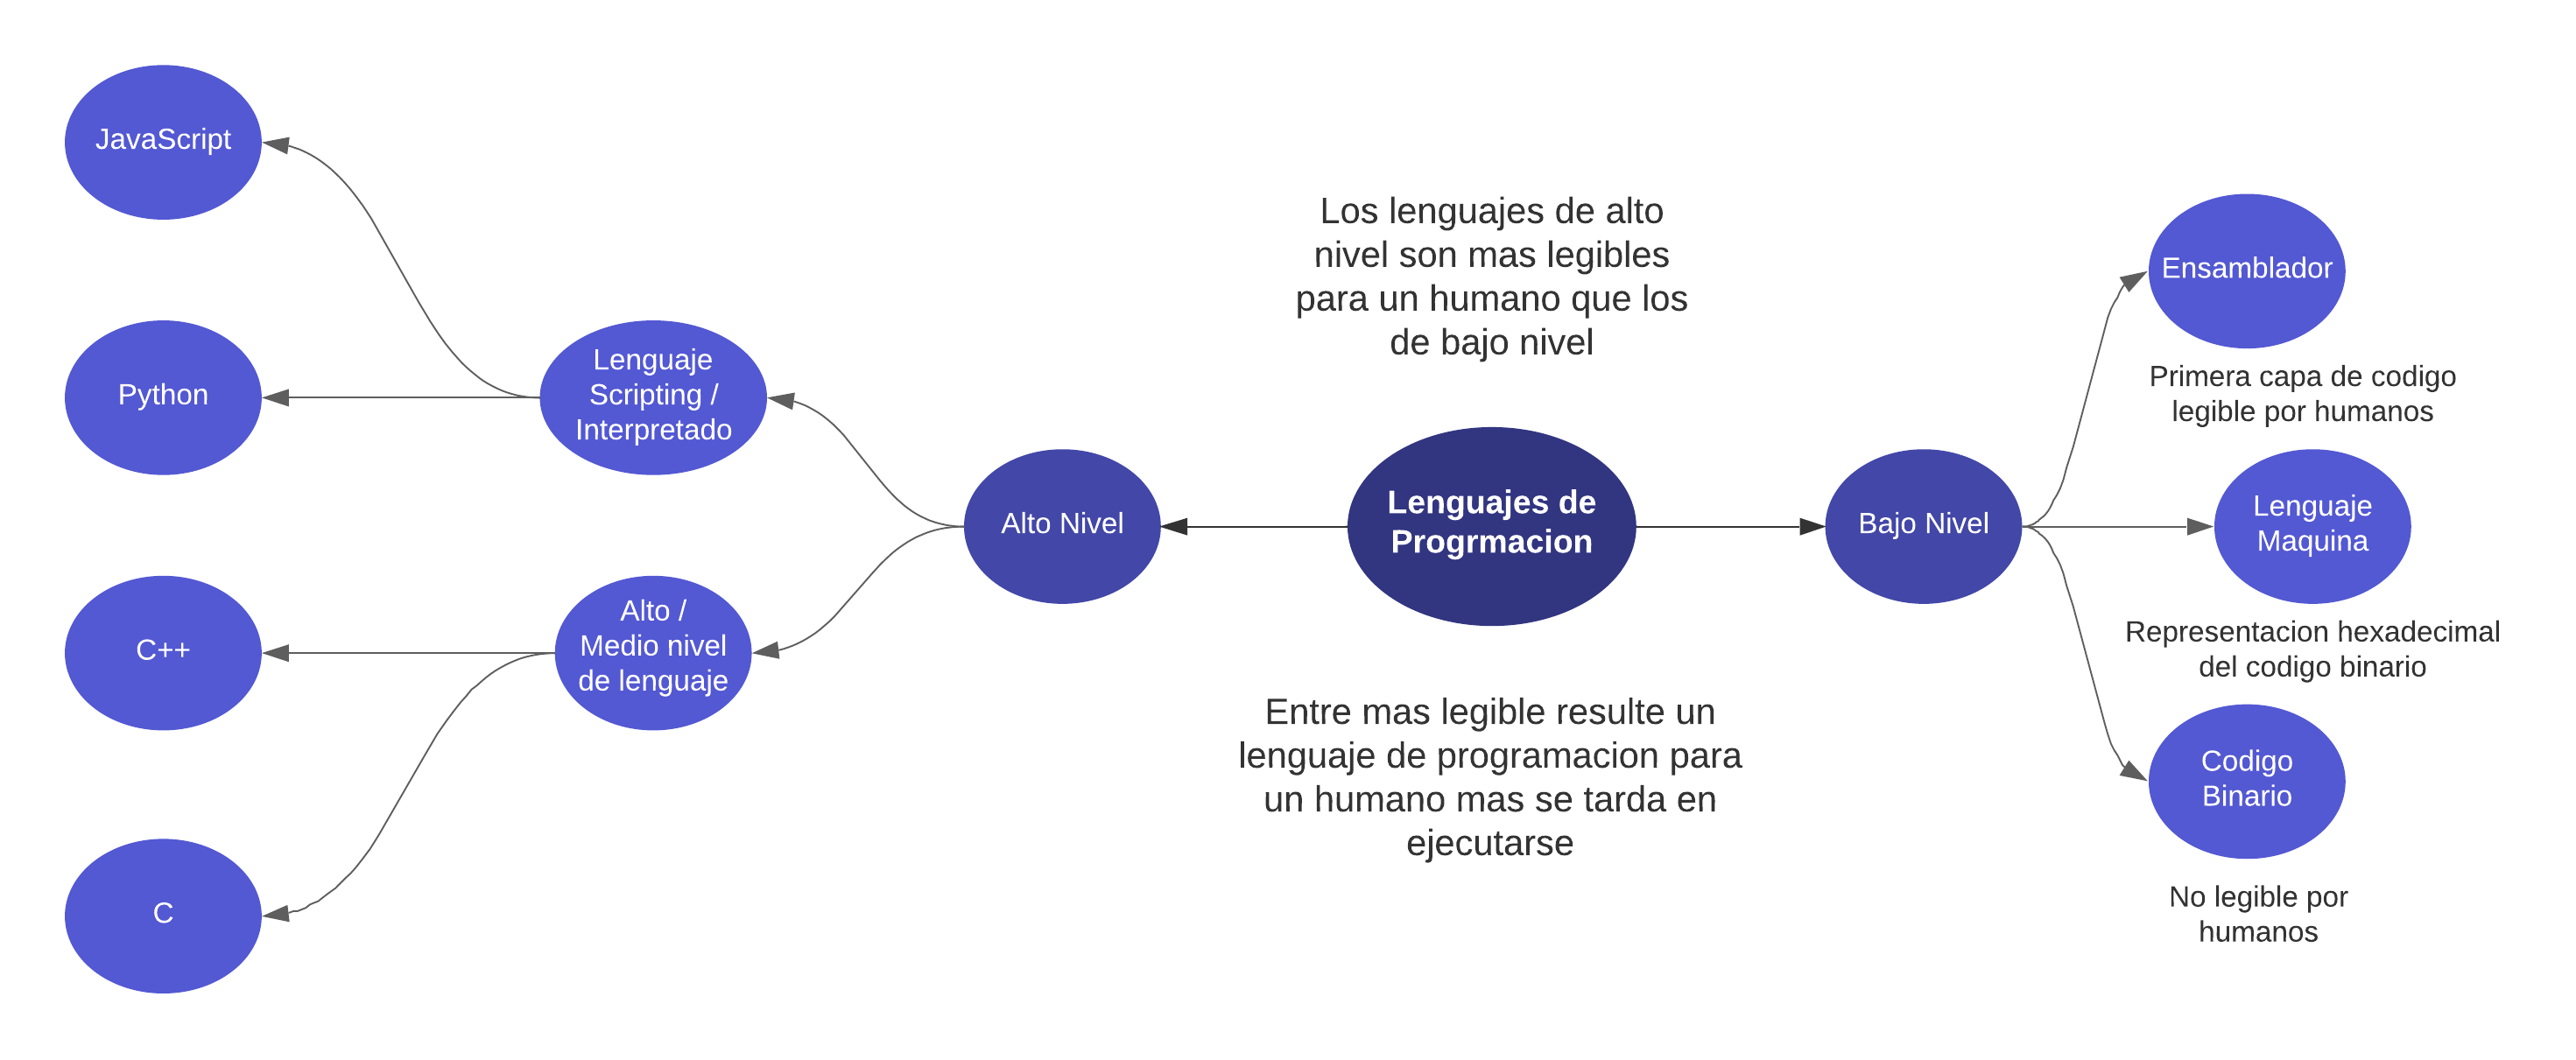
\includegraphics[scale = 0.7]{Comp _Pr1.png}
\end{center}

\newline

\textbf{2.} \textbf{(2.5pts.)} La siguiente gram\'atica genera expresiones en 
notaci\'on polaca inversa, es decir los argumentos preceden al operador:
\[
 E \to E\; E\; op \mid id \qquad \qquad op \to + \mid - \mid * \mid /
\]
Suponer que cada $id$ (identificadores en may\'usculas) tiene un atributo 
sint\'etico \texttt{name} que es una cadena y los s\'imbolos $E$ y $op$ tienen 
un atributo \texttt{val} que tambi\'en es una cadena.\\
Dise\~na una gram\'atica con atributos para organizar el atributo \texttt{val} 
de la ra\'iz del parse tree para guardar la traducci\'on de la expresi\'on en 
notaci\'on infija (utiliza los par\'entesis necesarios). 
Explica la idea que usas para definir las funciones sem\'anticas.\\
Por ejemplo, si las hojas del parse tree (de izquierda a derecha) son 
$A\; A\; B \; - \;* \; C \;/$ entonces la ra\'iz debe tener como atributo 
\texttt{val} la cadena $((A*(A-B))/C)$.\newline

\textbf{Solución:}
\begin{center}
  \begin{tabular}{| c | c |}
    \hline
    Producciones & Reglas Semánticas \\ \hline
    $S \rightarrow (E)$                  & $S.\code{val} :=$ $E$.\code{val} \\
    $E \rightarrow ((E_1)\: (E_2)\: op)$ & $E.\code{val} :=$ $E_1$.\code{val} $op$ $E_2$.\code{val}\\
    $E \rightarrow id$                   & $E.\code{name} :=$ $id$.\code{name}  \\
    $op \rightarrow +$                   & $op.\code{val} :=$ $+$  \\
    $op \rightarrow -$                   & $op.\code{val} :=$ $-$  \\
    $op \rightarrow *$                   & $op.\code{val} :=$ $*$  \\
    $op \rightarrow /$                   & $op.\code{val} :=$ $/$  \\ \hline
  \end{tabular}
\end{center}

A continuación se muestra el árbol para oganizar \code{val} respecto a $((A (A B -) *) C /)$:
\begin{center}
        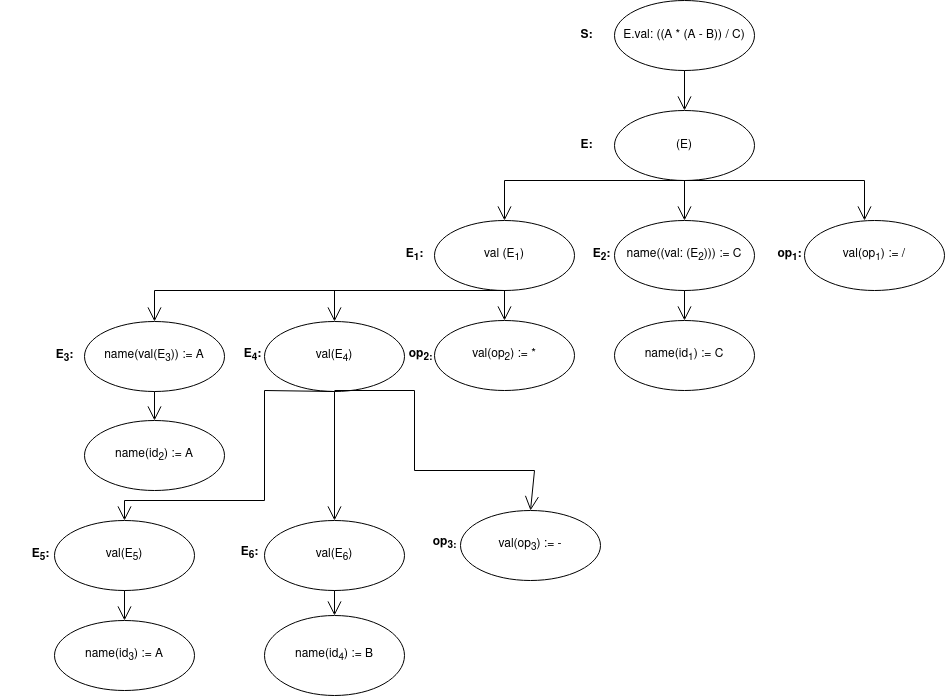
\includegraphics[width=.85\textwidth]{./02.png}
\end{center}
Cómo podemos notar, $S \rightarrow E = ((A * (A - B)) / C)$ que es generado por las reglas semánticas definidas. La
idea es ir aplicando recursión de hojas a raíz, y siguiendo las reglas de semánticas. De esta manera pasamos de
notación polaca inversa a sufija.

\newpage
%%% Pregunta 03:
Utilizando la tabla de traducci\'on entre una representaci\'on 
intermedia lineal y las instrucciones de arquitectura MIPS, 
genera el c\'odigo m\'aquina para la siguiente secuencia:

%%%%%%%%%%%%% TODO. Sebas, no sé que onda con el paquete, ya lo importé y nada.
% https://es.overleaf.com/learn/latex/Code_Highlighting_with_minted
% https://github.com/gpoore/minted/issues/70
%\begin{minted}[escapeinside=//]{c}
% d := c + 8
% a := a + b/$^{last}$/
% M[d/$^{last}$/] := a
% IF a < c THEN L1 ELSE L2
% LABEL L1
%\end{minted}

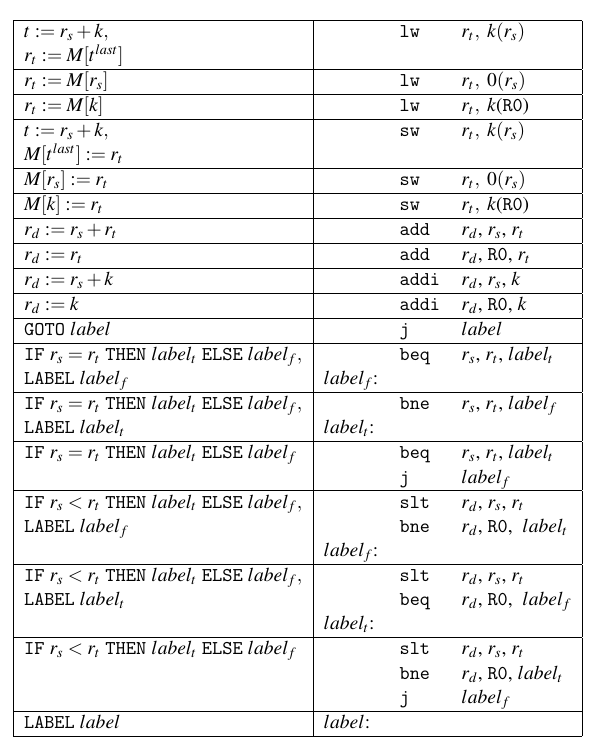
\includegraphics[width=.75\textwidth]{./MIPSInstrSet}

\newpage
\textbf{4.} \textbf{(2pts.)} Considera el siguiente fragmento de c\'odigo:
\begin{lstlisting}
if ( c[i] != 0 )
then 
   a[i] := b[i] / c[i];
else 
   a[i] := b[i];
\end{lstlisting}
Obtener las representaciones intermedias correspondientes a 1) \'arbol de 
sintaxis abstracta; 2) gr\'afica de control de flujo y 3) c\'odigo de tres 
direcciones. Explica tus respuestas. \\
Discutir (ampliamente) las ventajas que consideras para cada representaci\'on.

\newpage
\textbf{5.}Considera la siguiente gram\'atica:
\[
    \begin{array}{rcl}
        E & \to & -E \mid (E) \mid VE'\\
        E' & \to & -E \mid \varepsilon\\
        V & \to & \mathtt{id}V'\\
        V' & \to & (E) \mid \varepsilon\\
    \end{array}
\]
\begin{enumerate}

    \item Muestra el c\'alculo de los conjuntos {\ffst} y {\ffollow}.

        \begin{itemize}

            \item FIRST

            \begin{itemize}

                \item FIRST(E) = \{-, (, FIRST(V)\}

                \item FIRST(E') = \{-\}

                \item FIRST(V) = \{i\}

                \item FIRST(V') = \{(\}

            \end{itemize}

            \item FOLLOW

            \begin{itemize}

                \item FOLLOW(E) = \{FIRST(E), FIRST(E')\}

                \item FOLLOW(E') = \{FIRST(E)\}

                \item FOLLOW(V) = \{d\}

                \item FOLLOW(V') = \{FIRST(E)\}

            \end{itemize}

        \end{itemize}

    \item Muestra dos \'arboles de sintaxis, uno abstracta y otro
    concreta para la cadena
    $-\mathtt{id}(-\mathtt{id})-\mathtt{id}$.

        \begin{figure}[h]
            \centering
            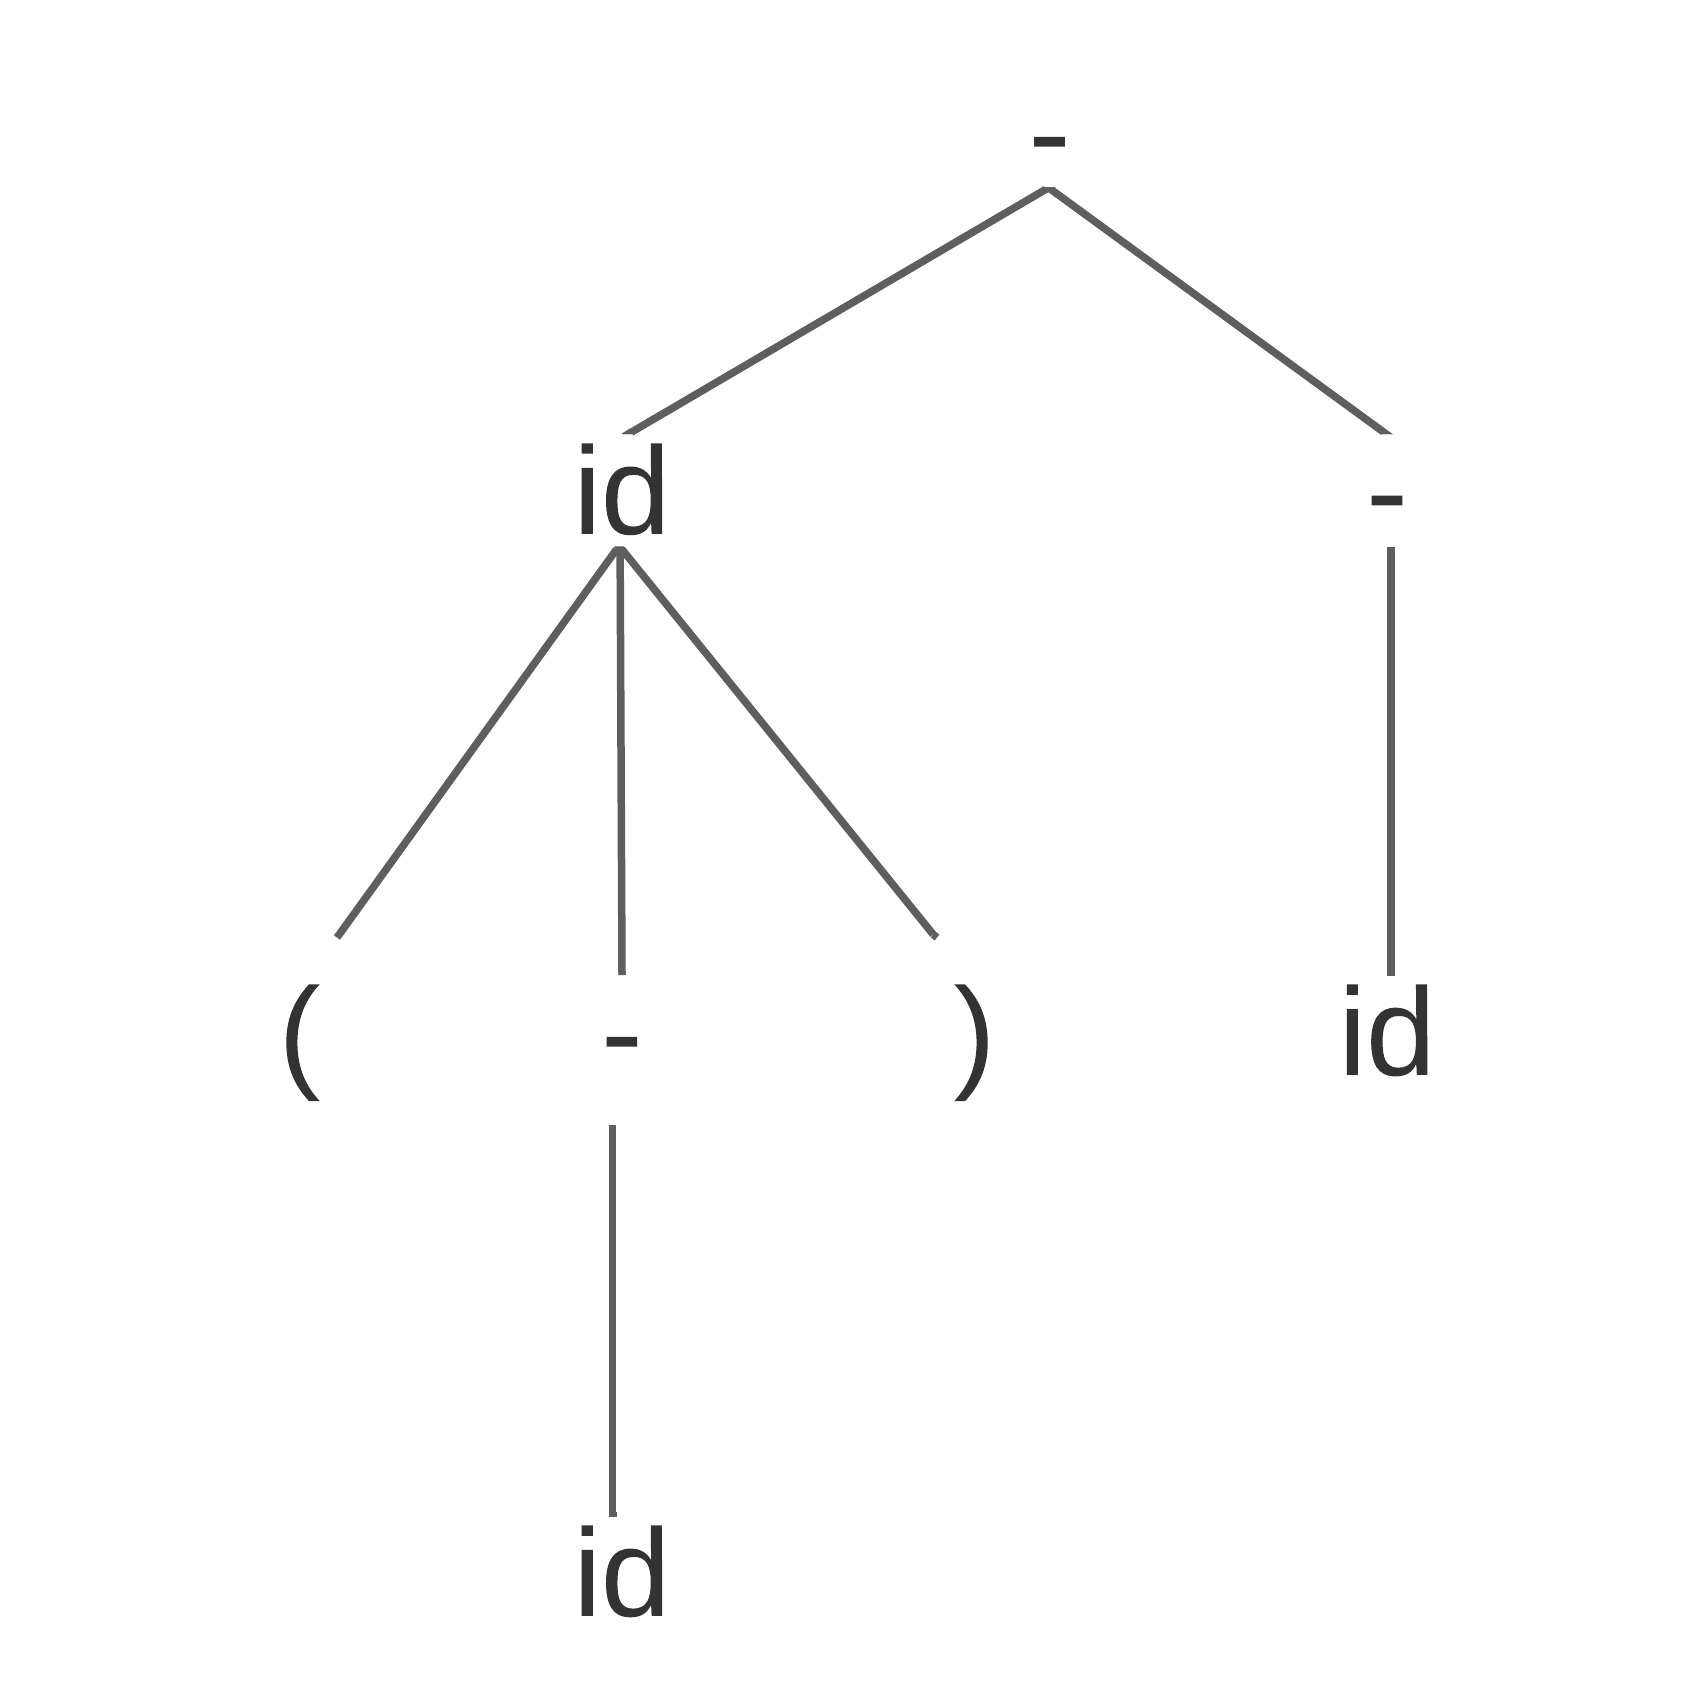
\includegraphics[scale = 0.5]{../Imagen/abst}
            \caption{Arbol de Sintaxis Abstracta}
            \label{fig:abst}
        \end{figure}


\end{enumerate}
\end{document}
